\section{Labels of the vertices}
%<-------------------------------------------------------------------------->
If no label is given, the label of a vertex is its name. The behavior of the
labels can be changed locally with the options of \tkzcname{Vertex}, or for
all the vertices with the macros of this section.

\subsection{Options of \tkzcname{Vertex} for the labels}

\subsubsection{Option \tkzname{L}}
\begin{tkzexample}[latex=7cm,small]
\begin{tikzpicture}
  \Vertex[L=$\alpha$]{a}
  \EA[unit=4](a){b}
\end{tikzpicture}
\end{tkzexample}

\subsubsection{Option \tkzname{Math}}
The label is written in math mode; there is no need to give \tkzname{L} in
math mode.

\begin{tkzexample}[latex=7cm,small]
\begin{tikzpicture}
  \Vertex[Math]{A_1}
  \Vertex[Math,L=\alpha,x=4,y=0]{a}
\end{tikzpicture}
\end{tkzexample}

\subsubsection{Option \tkzname{NoLabel}}
The label is not displayed. To remove the labels of all the vertices, use
\tkzcname{SetVertexNoLabel}.

\begin{tkzexample}[latex=7cm,small]
\begin{tikzpicture}
  \SetGraphUnit{4}
  \Vertex[NoLabel]{A}
  \EA[NoLabel](A){B}
\end{tikzpicture}
\end{tkzexample}

\subsubsection{Options \tkzname{LabelOut}, \tkzname{Lpos} and \tkzname{Ldist}}
The first option places the label outside the node, the second one gives
its direction (an angle) and the last one the distance between the label and
the node.

\begin{tkzexample}[latex=7cm,small]
\begin{tikzpicture}
  \Vertex[LabelOut]{A}
  \Vertex[LabelOut,Lpos=60,Ldist=.5cm,x=2,y=0]{B}
  \Vertex[LabelOut,Lpos=60,x=4,y=0]{C}
\end{tikzpicture}
\end{tkzexample}

\subsection{Macros for all the vertices}

\begin{NewMacroBox}{SetVertexNoLabel}{}
\emph{The labels of the next vertices are removed (option
\tkzname{NoLabel}).}
\end{NewMacroBox}

\begin{NewMacroBox}{SetVertexLabel}{}
\emph{The labels are displayed again.}
\end{NewMacroBox}

\begin{tkzexample}[latex=7cm,small]
\begin{tikzpicture}
  \SetVertexNoLabel
  \SetGraphUnit{2}
  \Vertex{A}     \EA(A){B}
  \SetVertexLabel  \EA(B){C}
\end{tikzpicture}
\end{tkzexample}

\begin{NewMacroBox}{SetVertexMath}{}
\emph{The labels are written in math mode (option \tkzname{Math}). The
macro also applies to the graphs of \tkzname{tkz-berge}.
\tkzcname{SetVertexNoMath} cancels it.}
\end{NewMacroBox}

\begin{tkzexample}[latex=7cm,small]
\begin{tikzpicture}
  \SetVertexMath
  \Vertex{A_1}  \EA[unit=3](A_1){A_2}
\end{tikzpicture}
\end{tkzexample}

\begin{NewMacroBox}{SetVertexLabelOut}{}
\emph{The labels are placed outside the vertices (option \tkzname{LabelOut});
\tkzname{Lpos} and \tkzname{Ldist} give their position.
\tkzcname{SetVertexLabelIn} writes the labels inside the vertices again.}
\end{NewMacroBox}

\begin{tkzexample}[latex=7cm,small]
\begin{tikzpicture}
  \SetGraphUnit{3}
  \SetVertexLabelOut
  \Vertex{A}  \EA(A){B}
  \SetVertexLabelIn  \SO(B){C}
\end{tikzpicture}
\end{tkzexample}

These macros act until the end of the current group (a \tkzname{scope}
environment, a \tkzname{tikzpicture} or braces).

\endinput
